% begin module volumes-washer
\begin{frame}
\begin{example}[Typical Cross-Section is a Washer]
\begin{columns}[c]
\column{.35\textwidth}
\psset{xunit=1cm, yunit=1cm}
\begin{pspicture}(-1,-1)(1,1)
\tiny%
\renewcommand{\fcScreenStyle}{x}%
\renewcommand{\fcScreen}{[0 0 -1] 0}%
\renewcommand{\fcIterationsU}{4}%
\fcBoundingBox{-1.8}{-1.8}{1.8}{1.8}
\only<3->{\renewcommand{\fcScreen}{[-0.05 -0.05 -1] 0}}%
\only<4->{\renewcommand{\fcScreen}{[-0.1 -0.1 -1] 0}}%
\only<5->{\renewcommand{\fcScreen}{[-0.15 -0.15 -1] 0}}%
\only<6->{\renewcommand{\fcScreen}{[-0.2 -0.2 -1] 0}}%
\only<7->{\renewcommand{\fcScreen}{[-0.25 -0.25 -1] 0}}%
\fcStartIIIdScene%
\only<3->{\fcPutIIId{[-0.1 -0.1 1.6]}{$z$}}%
\fcAxesIIIdInScene[arrows=->, xLabel={$x$}, yLabel={$y$},zLabel={} ]{1.5}{1.5}{1.5}%
\fcFinishIIIdScene
\end{pspicture}

\only<handout:0| 1>{%
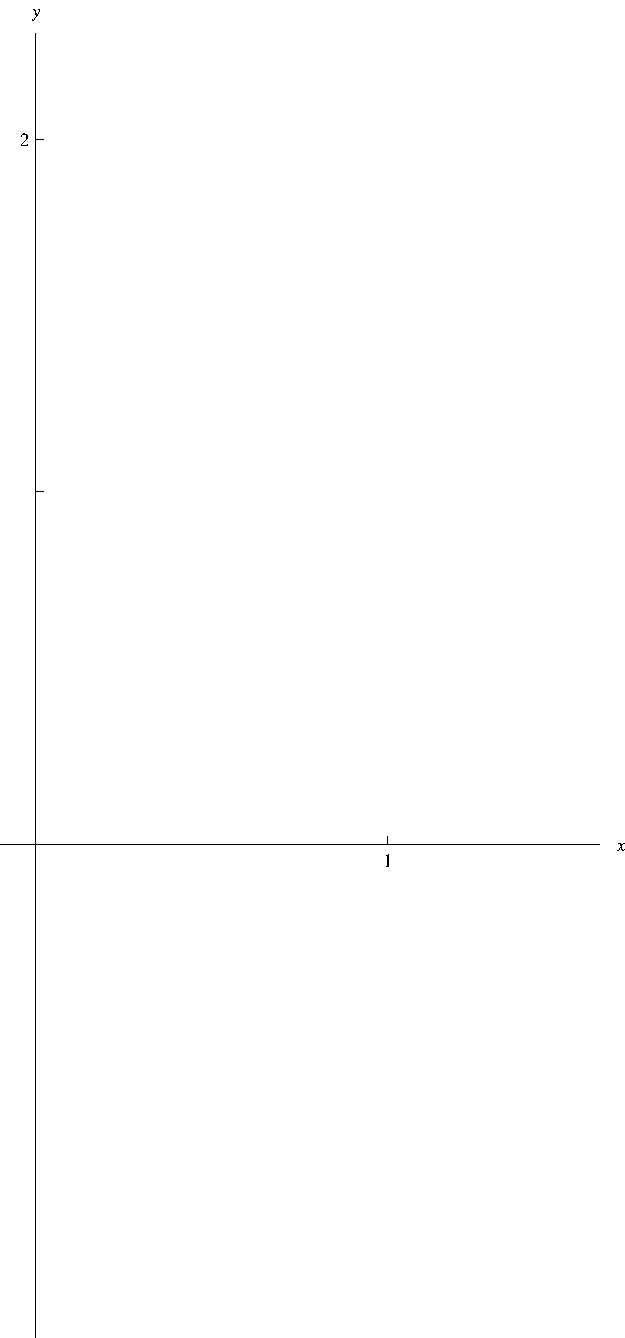
\includegraphics[height=3.3cm]{volumes/pictures/06-02-washera.pdf} %
}%
\only<handout:0| 2>{%
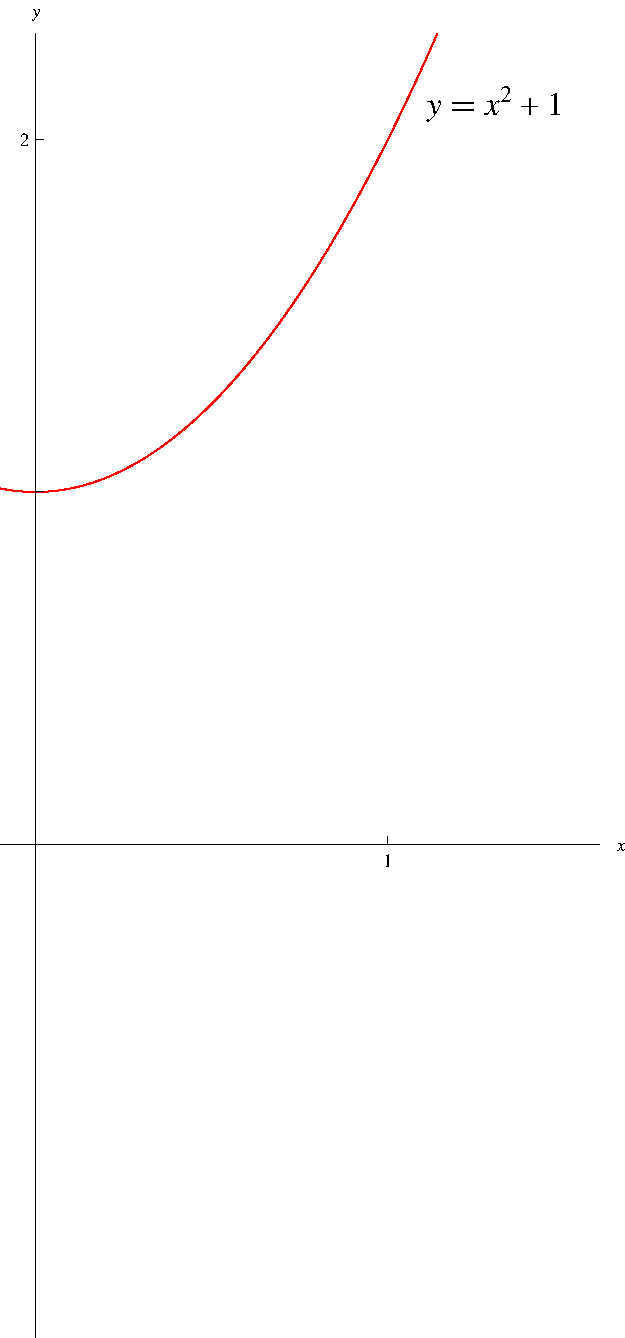
\includegraphics[height=3.3cm]{volumes/pictures/06-02-washerb.pdf} %
}%
\only<handout:0| 3>{%
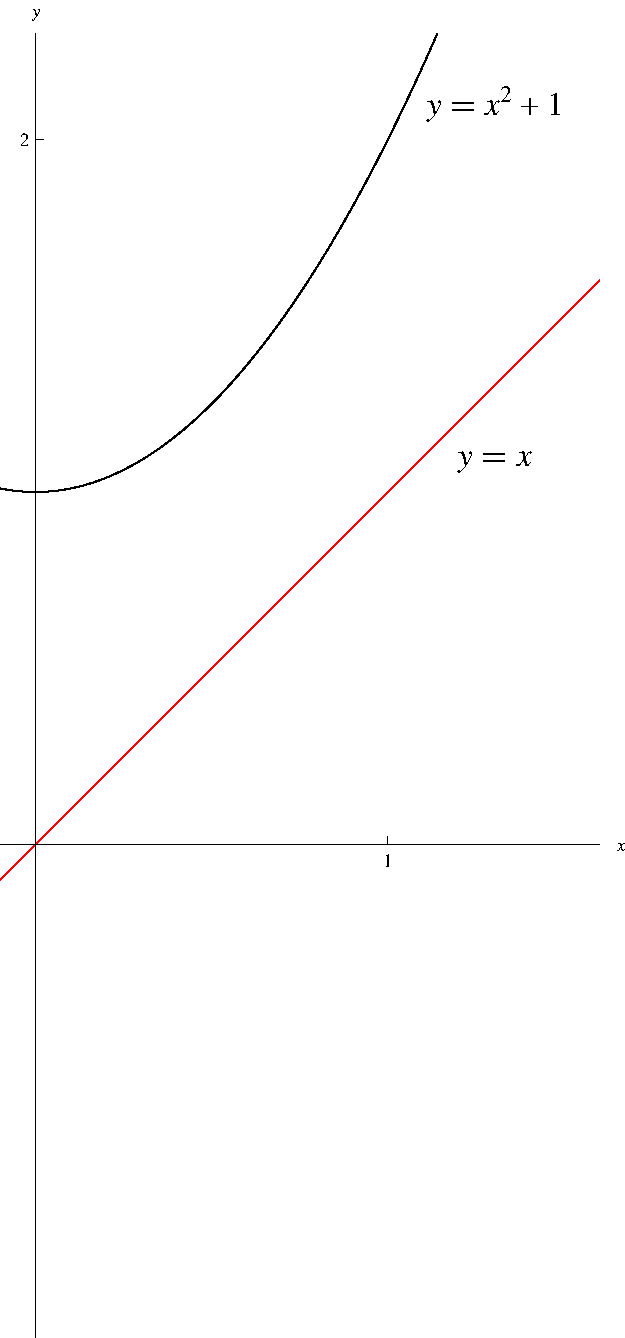
\includegraphics[height=3.3cm]{volumes/pictures/06-02-washerc.pdf} %
}%
\only<handout:0| 4>{%
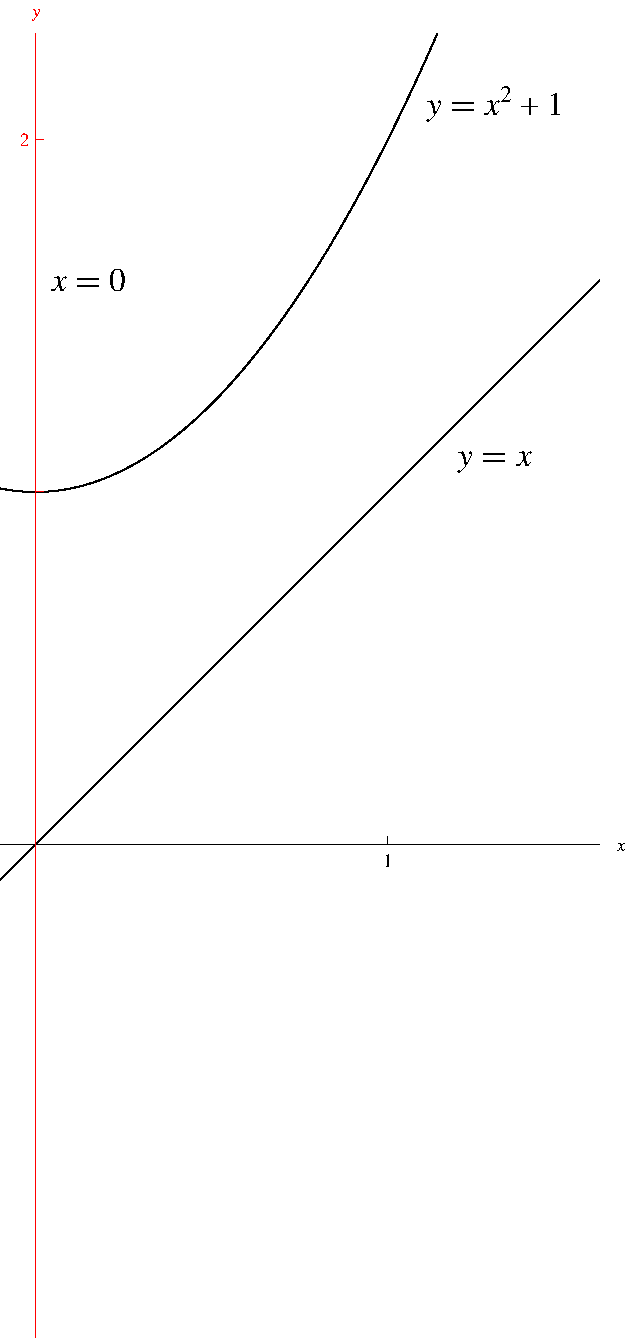
\includegraphics[height=3.3cm]{volumes/pictures/06-02-washerd.pdf} %
}%
\only<handout:0| 5>{%
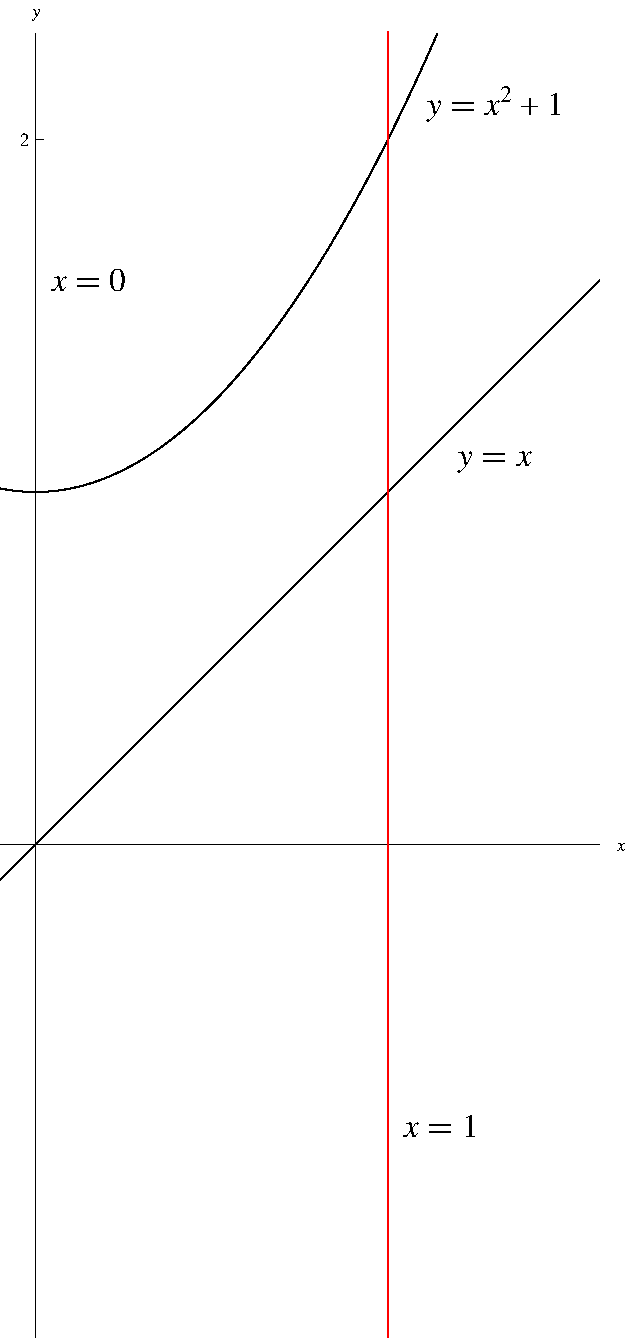
\includegraphics[height=3.3cm]{volumes/pictures/06-02-washere.pdf} %
}%
\only<handout:0| 6>{%
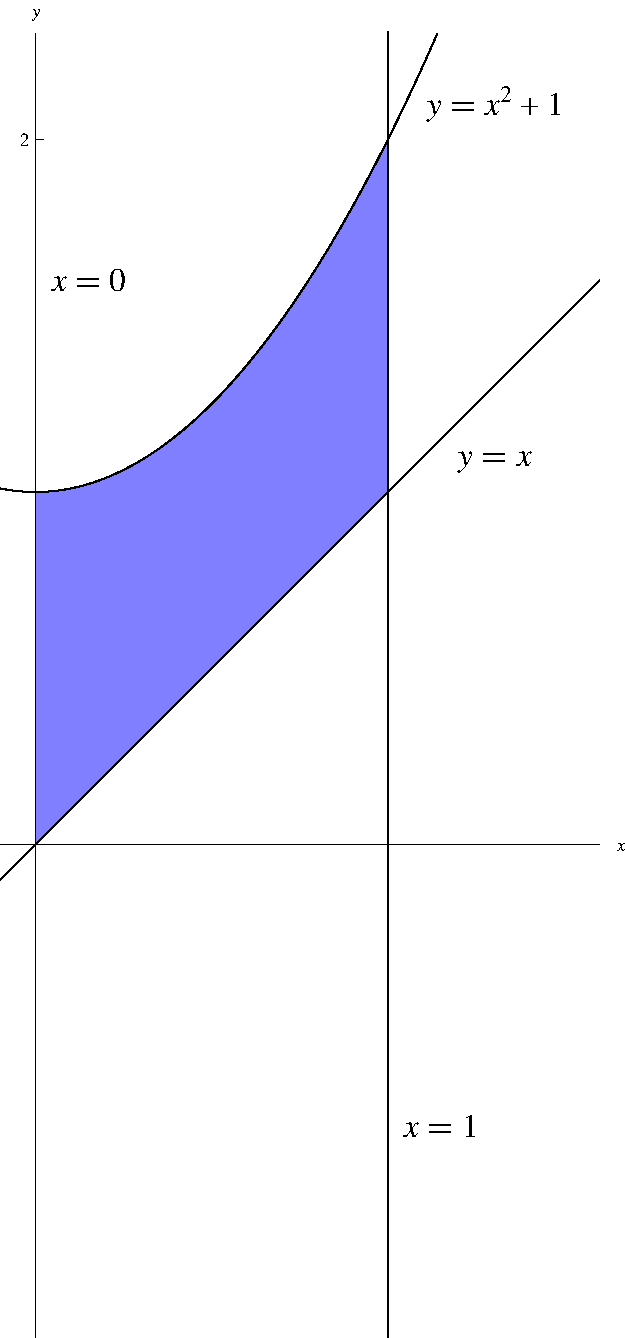
\includegraphics[height=3.3cm]{volumes/pictures/06-02-washerf.pdf} %
}%
\only<7->{%
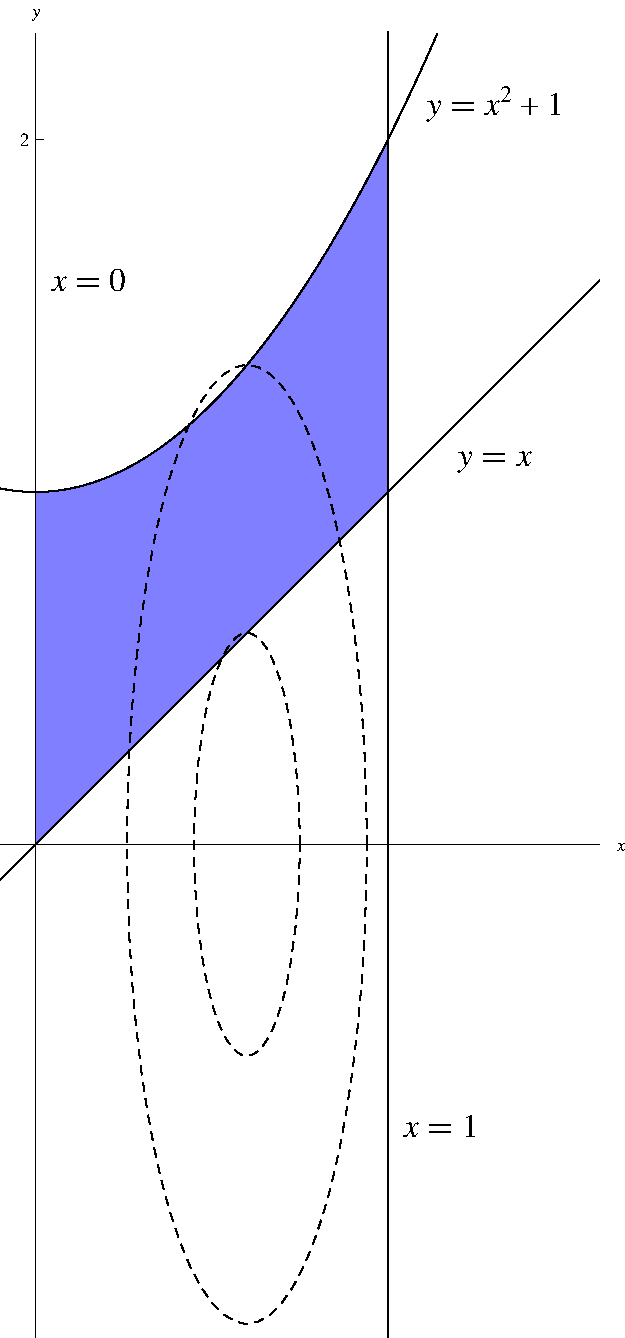
\includegraphics[height=3.3cm]{volumes/pictures/06-02-washerg.pdf} %
}%

\column{.65\textwidth}
Find the volume of the solid obtained by rotating about the $x$-axis \alert<handout:0| 6>{the region bounded by \alert<handout:0| 2>{$y = x^2+1$}, \alert<handout:0| 3>{$y = x$}, \alert<handout:0| 4>{$x = 0$}, and \alert<handout:0| 5>{$x = 1$}}.

\uncover<7->{%
The typical cross-section is a washer centered at $(x, 0)$.
}%

\uncover<8->{%
\alert<handout:0| 8-9>{Area of the inner circle: \uncover<9->{$\pi x^2$}}

\alert<handout:0| 10-11>{Area of the outer circle: \uncover<11->{$\pi (x^2+1)^2$}}
}%
\abovedisplayskip=0pt
\belowdisplayskip=0pt
\abovedisplayshortskip=0pt
\belowdisplayshortskip=0pt
\begin{align*}
\uncover<12->{%
V%
}%
& \uncover<12->{ = } %
\uncover<12->{%
\int_0^1 \left( \pi (x^2+1)^2 - \pi x^2    \right) \ \diff x%
}\\%
& \uncover<13->{ = } %
\uncover<13->{%
\pi \int_0^1 \left( \alert<handout:0| 14-15>{x^4} + \alert<handout:0| 16-17>{x^2} + \alert<handout:0| 18-19>{1} \right) \  \diff x%
}\\%
& \uncover<14->{ = } %
\uncover<14->{%
\pi \left[ \alert<handout:0| 15>{\uncover<15->{\frac{x^5}{5}}} + \alert<handout:0| 17>{\uncover<17->{\frac{x^3}{3}}} + \alert<handout:0| 19>{\uncover<19->{x}} \right]_0^1%
}\\%
& \uncover<20->{ = } %
\uncover<20->{%
\pi \left( \frac{1}{5} + \frac{1}{3} + 1\right) \uncover<21->{= \frac{23}{15}\pi}
}%
\end{align*}
\end{columns}
\end{example}
\end{frame}
% end module volumes-washer
